% \epigraph{Father Dougal: Didn't you tell me once that Father Jack had a trial for Liverpool?
% \\ Father Ted: No... no, he was on trial, in Liverpool.}
\chapter{Introduction}
\vspace{-5in}

\includegraphics[height=2.0in]{thesis/latex/st_a_logo_.png}
\vspace{3in}

\epigraph{Galaxies are funny old things. Broadly characterised into being red or blue, the basics of galaxy properties are relatively simple. The deeper we dig, however, the more nuance and subtleties we unveil. On smaller scales galaxies act as astronomic laboratories shedding light on the evolution of stars and gas, while on cosmological scales these baryonic building blocks trace the large scale structure of the Universe, revealing the nature of gravity.}

\label{ch:intro}
\section{Galaxy evolution} \label{sec:gal_evo_intro}
Its pretty tricky to make an all encompassing model for the Universe. Nevertheless, our best guess is the $\Lambda$ cold dark matter ($\Lambda$CDM) paradigm. In this framework, the are three main ingredients to the Universe; a cosmological constant ($\Lambda$) labelled dark energy, required for the late time accelerated expansion; cold dark matter (CDM) providing the `missing' gravity; and the matter we can see, baryons. 

The early Universe is to first order homogeneous, however, minute quantum fluctuations in the density field grow linearly to form small haloes of dark matter. Structure growth is naturally hierarchical where these small haloes of dark matter progressively merge to form the more massive structures at later times \citep{press1974}. Galaxies form in the potential wells of the dark matter haloes through the gravitational collapse of gas, which in turn radiatively cools and goes on to form stars \citep{white1978}. The assembly and merger history of these haloes is intimately linked to the evolution of its baryonic components and hence the characteristics of the galaxy we observe in the local Universe.

\subsection{Tuning in}
One of the most powerful methods of understanding a galaxy is its visual form, often referred to as morphology. In the local Universe, the morphological diversity that galaxies can posses is remarkable. The first effort to characterise this (albeit before the label of `\textit{galaxy}') was devised by Edwin Hubble who separated galaxies based on their key features \citep{hubble1926, hubble1936}. Known colloquially as the `tuning fork', Hubble divided galaxies into a classification scheme based on their overall shape (i.e. ellipsoidal, spheroidal or disk/flattened), prevalence of a bulge (i.e. is the overall shape dominated by the disk or the bulge?), the presence of bar structure, and the structure of spiral arms. An example of the `tuning fork' is given in Figure \ref{fig:hubble_fork} and the distinct categories can be described as follows:

\begin{itemize}
    \item \textbf{Ellipticals (E):} Elliptical galaxies are the most visually mundane, demonstrating smooth, often featureless morphologies. Unsuprisingly their eponym derives from their elliptical shape; ranging from round (E0) to the most flattened (E7). Moving to the right of the diagram, ellipticals typically display faint substructure such as disks. For the most part, ellipticals host very little gas, dust, and are made up mostly of older, redder stars. In generality they make up the `red' bucket of galaxy bi-modality.
    
    \item \textbf{Spirals (S):} The poster child of galaxy evolution, spiral galaxies are distinguished by a flattened, disk shape. They display vivid substructure with winding spiral arms of young, blue stars and gas which encompass a central bulge of older, redder stellar populations. Sub-classification of spirals is determined by the degree of winding of their spiral arms; ranging from grand-design (Sa) to flocculent (Sc). In simpler terminology this refers to going from the most tightly wound spiral arms with the largest bulges to the loosest with the smallest bulges. These galaxies are typically gas rich and are continuing to form stars at a high rate. 
    
    \item \textbf{Barred Spirals (Sb):} A subtle twist on disky galaxies, barred spirals demonstrate spiral arms that originate from a distinct central rectangularly shaped bar. Similarly they are defined (left to right) based on the prominence of their central bulge and \textit{flocculation}.
    
    \item \textbf{Lenticular (S0):} Falling in the middle of this is the wonderful amalgamation of the lenticular galaxy. In parallel to ellipticals, they consist of a bright central bulge, however are surrounded by an extended disk-like structure. In contrast to the disks of spirals, there is no obvious spiral structure and they are forming stars at intermediate rates.
    
    \item \textbf{Irregular (Irr):} The sequence outcast, Irregular galaxies demonstrate no regular structure (i.e. no disk or smooth and spheriodal shape). These galaxies are typically visually disturbed and asymmetric, sometimes containing `bursty' regions of star formation. 
\end{itemize}

\begin{figure}
	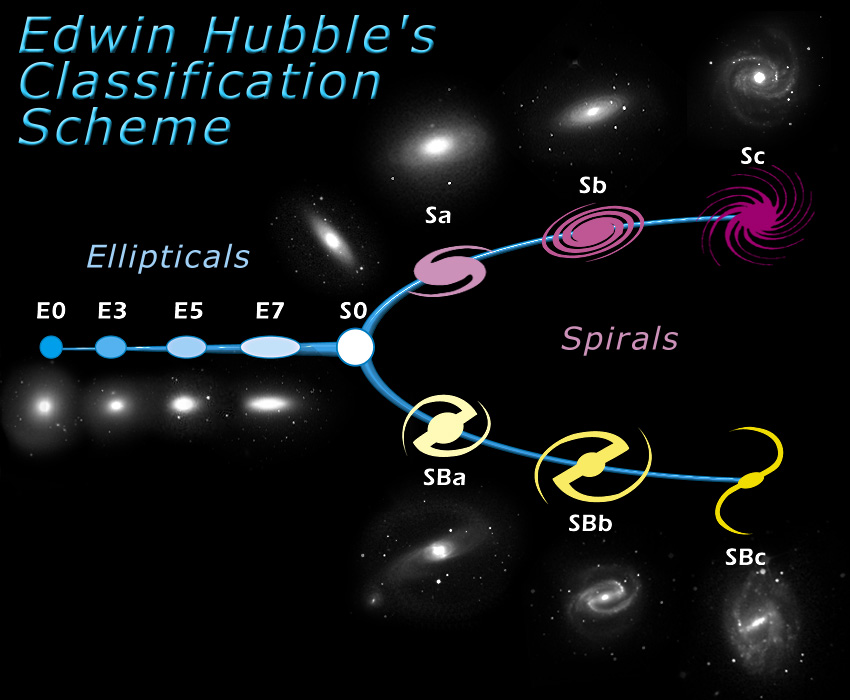
\includegraphics[width=\linewidth]{thesis/latex/introduction/hubble_tuning_fork.jpg}
    \caption{Illustration of the Hubble sequence with an example galaxy image for each distinct classification. Credit: NASA / ESA.}
    \label{fig:hubble_fork}
\end{figure}

\subsection{Large scale redshift surveys}
In the past few decades, extensive galaxy surveys such as the Sloan Digital Sky Survey \citep[SDSS,][]{york2000} and the Galaxy And Mass Assembly survey \citep[][]{driver2009} have provided a wealth of spectroscopic and photometric information for 100,000s of galaxies. The sheer wealth of photometric information has enabled tremendous collaboration between the public and scientists through the Galaxy Zoo project \citep[e.g.][]{lintott2008, lintott2011, willett2013}, taking the number of visually classified galaxies into the millions. In parallel, developments in computational techniques and the use of a combination of photometric with spectroscopic information have enabled systematic investigation of a whole host of galaxy structural properties. Stellar populations, star formation histories and sizes are all fundamental properties used to understand a galaxy's evolution. 

\subsection{Local environment}
\red{talk about galaxy bi-modality, the ability to accrete gas to maintain star formation and how this relates to local environment.} Despite this diversity in optical morphology, galaxies can be broadly classified into two distinct types, which populate different regions of colour-mass diagrams. The first category, called the red sequence, is populated by galaxies of redder colour and smoother structure, inherent of ellipticals and lenticulars. The second, the blue cloud, are populated by galaxies with bluer stellar populations and typically host a disk, characteristic of spirals. Galaxies populate this distribution in an entirely bi-modal nature, with very few bridging the intermediate region between the red sequence and blue cloud which is referred to as the `green valley'. The division of galaxies into these sub-categories is intimately related to a given galaxy's supply of gas. 

The ability for a galaxy to continue to accrete gas and hence form stars, is dependent on the type of environment that a galaxy resides. Unsurprisingly, many galaxies do not exist in isolation. On small scales, galaxies can be found in groups: the Milky Way, our neighbour Andromeda, and other smaller nearby galaxies being one such example, called the Local Group. The local environment in which a galaxy occupies is quantified by the size of the group (or cluster) in terms of mass, or number of galaxies.

We find that redder early-type galaxies are more common in large galaxy groups and clusters, whereas bluer late-type galaxies are more isolated, preferentially residing in field-like regions \citep[e.g.][]{dressler1980, whitmore1993}. This can be understood through the prevalence or effectiveness of different physical processes in each regime, which in turn modulate galaxy properties. In rich cluster environments, processes which remove or restrict gas in-flow (and hence suppress star formation) are common; such as ram pressure stripping \citep[e.g.][]{gunn1972} or harrassment \citep[e.g.][]{moore1996}. Adding to the cacophony are suffocation and strangulation \citep[e.g.][]{larson1980}, processes in addition to mergers and halo-gas stripping which act most strongly in less dense regimes. The richness of galaxy systems, or haloes, is crucial in understanding how the morphology of a galaxy will evolve.

\subsection{The cosmic web}
On large scales, galaxies and their constituent groups are part of a larger pattern, called the cosmic web. The same extensive galaxy surveys giving such insight to galaxy evolution, unveiled this web-like structure \citep[e.g.][]{delapparent1986, colless2001, tegmark2004} which consists of large filamentary structures which connect the high density peaks, observationally referred to as galaxy groups or clusters. At the other end of the scale, nearly empty void regions are encased by sheet-like walls, themselves a prediction from anisotropic collapse of the initial perturbations of the matter density field \citep{zeldovich1970, shandarin1989}. The filaments frame the walls at the points of their intersection, creating a framework for baryonic material to move from low density environments to hierarchically higher density. An example of the large scale structure traced by the positions of galaxies is given in Figure \ref{fig:cosmo_web_tng}.
\red{introduce sdss, introduce manga, introduce tng, introduce disperse}

\begin{figure}
	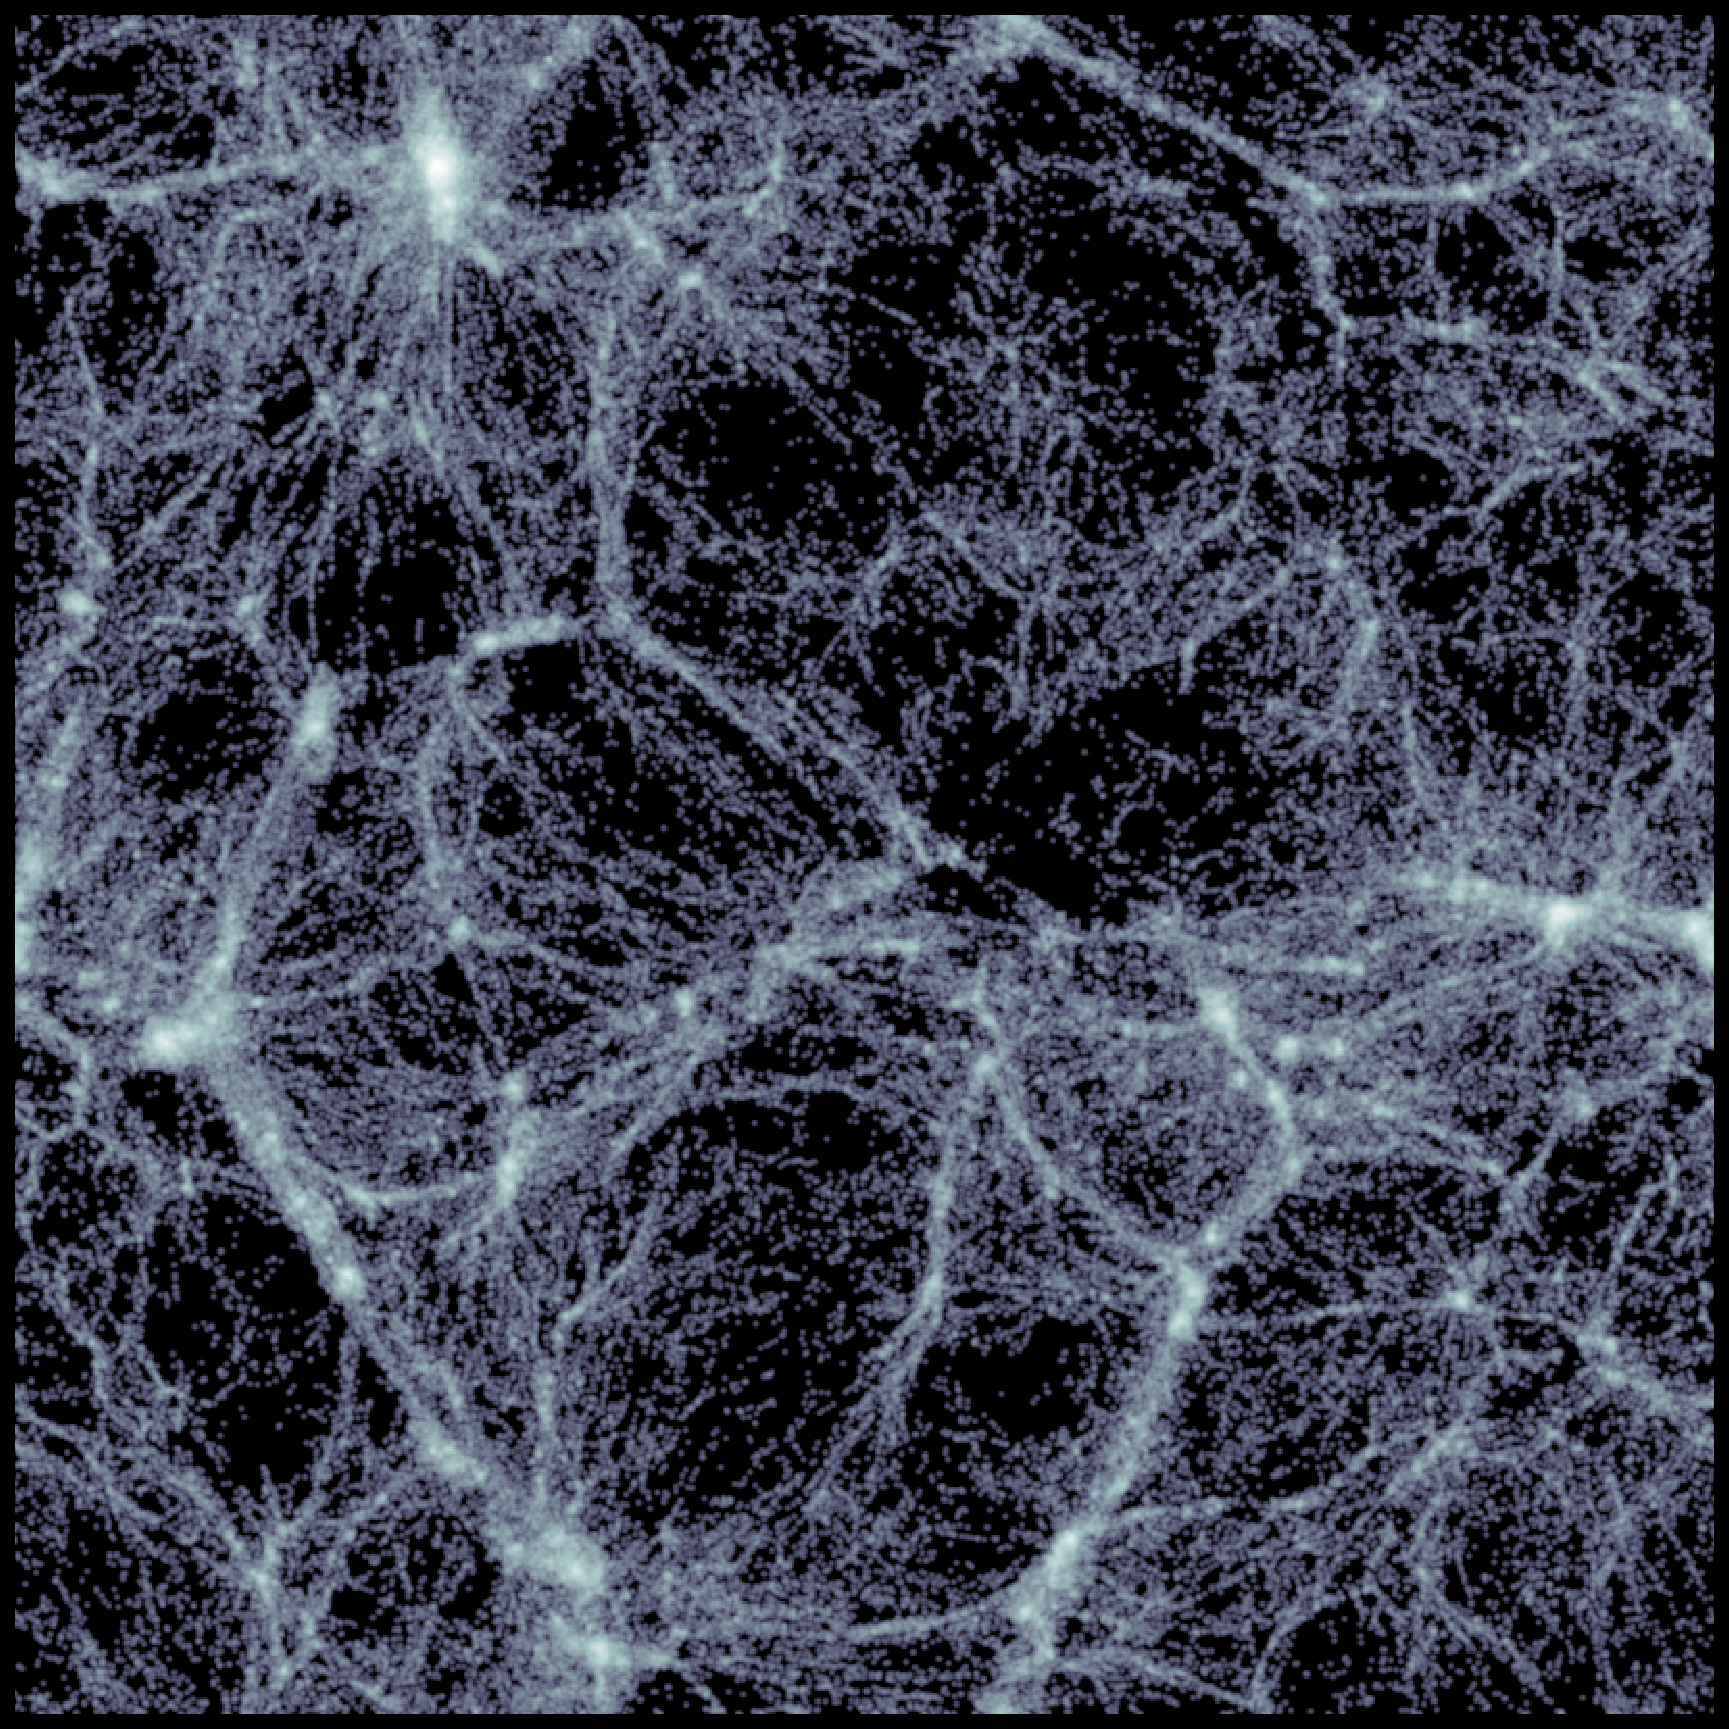
\includegraphics[width=\linewidth]{thesis/latex/introduction/slice_image_bone.pdf}
    \caption{Distribution of galaxies in the IllustrisTNG100 simulation. Galaxies naturally trace the anisotropic nature of large scale structure formation, with large filamentary networks on multiple scales connecting the overdensities and encasing the underdensities. Colour scale goes from dark to light corresponding to low to high densities of galaxies.}
    \label{fig:cosmo_web_tng}
\end{figure}

\subsubsection{The numerics of the cosmic web}
Despite the innate beauty of large scale structure, by its very nature it is complex and multi-scale. Understanding the relationship between the properties of galaxies and the cosmic web is reliant on building a mathematical framework to classify and identify distinct regions (voids, walls, filaments, nodes). This framework must be applicable to both observations and simulations making use of the large scale density field, reconstructed directly from the distribution of resolution elements (tracers; which can be DM particles or gas cells in simulations, or whole galaxies in both observations and simulations). 

There is no \textit{correct} choice in how we chose to mathematically characterise the cosmic web. Methods that succeed in some areas are naturally less sensitive in others, and what we \textit{should} aim to recover is as much a philosophical debate as it is a mathematical one. Different cosmic-web classifiers have often been designed with different cosmological questions in mind, and hence agreement is not \textit{necessarily} expected. Despite this, one common theme is that different methodologies associate a given web environment with similar density regimes (i.e. going from the most over-dense regimes associated with knots/clusters to the most under-dense with voids) \citep{libeskind2018}. Here we discuss two commonly considered techniques to recover large scale structure.

The first of which directly relies on the cosmic web being a product of the influence of large-scale tidal forces, by computing the \textit{tidal tensor} which acts as a method for quantifying the directionality of collapse and hence the anisotropy of the environment. In observations, the idea is to estimate the tidal tensor from a smoothed distribution of galaxy density, and at every given sampling point, compute the eigenvalues in each cartesian direction. Regions are then classified based the value of each eigenvalue with respect to a given threshold so that; void if all eigenvalues below threshold (no collapse), sheet (wall) if one eigenvalue above the threshold, a filament if two eigenvalues are above the threshold, and a knot (node) if all eigenvalues are above the threshold (collapse in all directions) \citep[e.g.][]{eardley2015}. The power in this method is the ability to characterise all regions of space, however, is faced with the difficulty that a specific smoothing scale must be chosen.

A methodology that is \textit{somewhat} agnostic to scale (or smoothing length) are geometric ridge extractors. Similar to tracing out the interconnection between peaks, valleys and everything in-between of a mountain range, ridge extractors classify the cosmic web based on the gradient of the density field. A popular choice at the time of writing (and the choice throughout this thesis) is the Discrete Persistent Structures Extractor \citep[DisPerSE][]{sousbie2011a, sousbie2011b}. The geometric three-dimensional ridge extractor can be applied directly to discrete data (i.e. point like distributions, meaning that it is well suited to astrophysical applications such as galaxy positions in large scale redshift surveys \citep[e.g.][]{malavasi2017, kraljic2018}.

Starting with a set of discrete points that can act to trace out the large scale density field, the first step in the process is to transform this into a density field. In the framework of DisPerSE this is typically done through using a Delaunay Tessellation to triangulate the space based on the local vicinity of neighbouring points. Specifically the Delaunay Tessellation Field Estimator technique \citep[DTFE;][]{schaap2000, cautun2011} is the default, however, any estimation of the density field can be used. 

DisPerSE is grounded in Morse-Smale theory which geometrically segments the density field into manifolds corresponding to individual morphological components of the cosmic web. Two key components of Morse theory (that correspond to physical elements of the cosmic web) are the ideas of critical points and integral (field) lines. \red{add diagram on manifolds etc?} Critical points correspond to the points in the density field where the gradient is zero. In three dimensional space, there are four different types of critical points as defined by their critical index. Minima have a critical index of 0 and maxima have a critical index of 3, with intermediate critical points referred to as saddles. Connecting the critical points are curves tangent to the gradient field which permeate of the density space (i.e. integral lines). By definition gradient lines start and end at critical points, and cannot overlap, meaning that space is tessellated into manifolds. A manifold is defined by the singular critical point where all integral field lines originate from and is enclosed by the critical points that the same integral lines terminate at. The complete set of such manifolds which segment the space is called the \textit{Morse complex} of the function. Each manifold is labelled accordingly to the order of critical points that populate it and hence correspond to different features of the cosmic web; i.e. ascending manifolds of dimension 3, 2, 1 and 0 as voids, walls, filaments and nodes of the cosmic web, respectively. 

A common difficulty is how to define how robust certain classified structures are. Using sparsely sampled data sets such as galaxy surveys, a quantification of the significance of the identified morphological features must be made with respect to shot noise. Here, this is dealt with through use of a \textit{persistence ratio} which measures the significance of topological connection between individual pairs of critical points (i.e. you can visualise this as the difference between two tall distinct mountains and a small boulder on the side of a single mountain). This mimics an adaptive smoothing depending on the local level of noise. In practice, this threshold is expressed in term of number of $\sigma$. \red{add sigma diagram and analogy with the boulder on a hill?}

\begin{figure*}
    \centering
	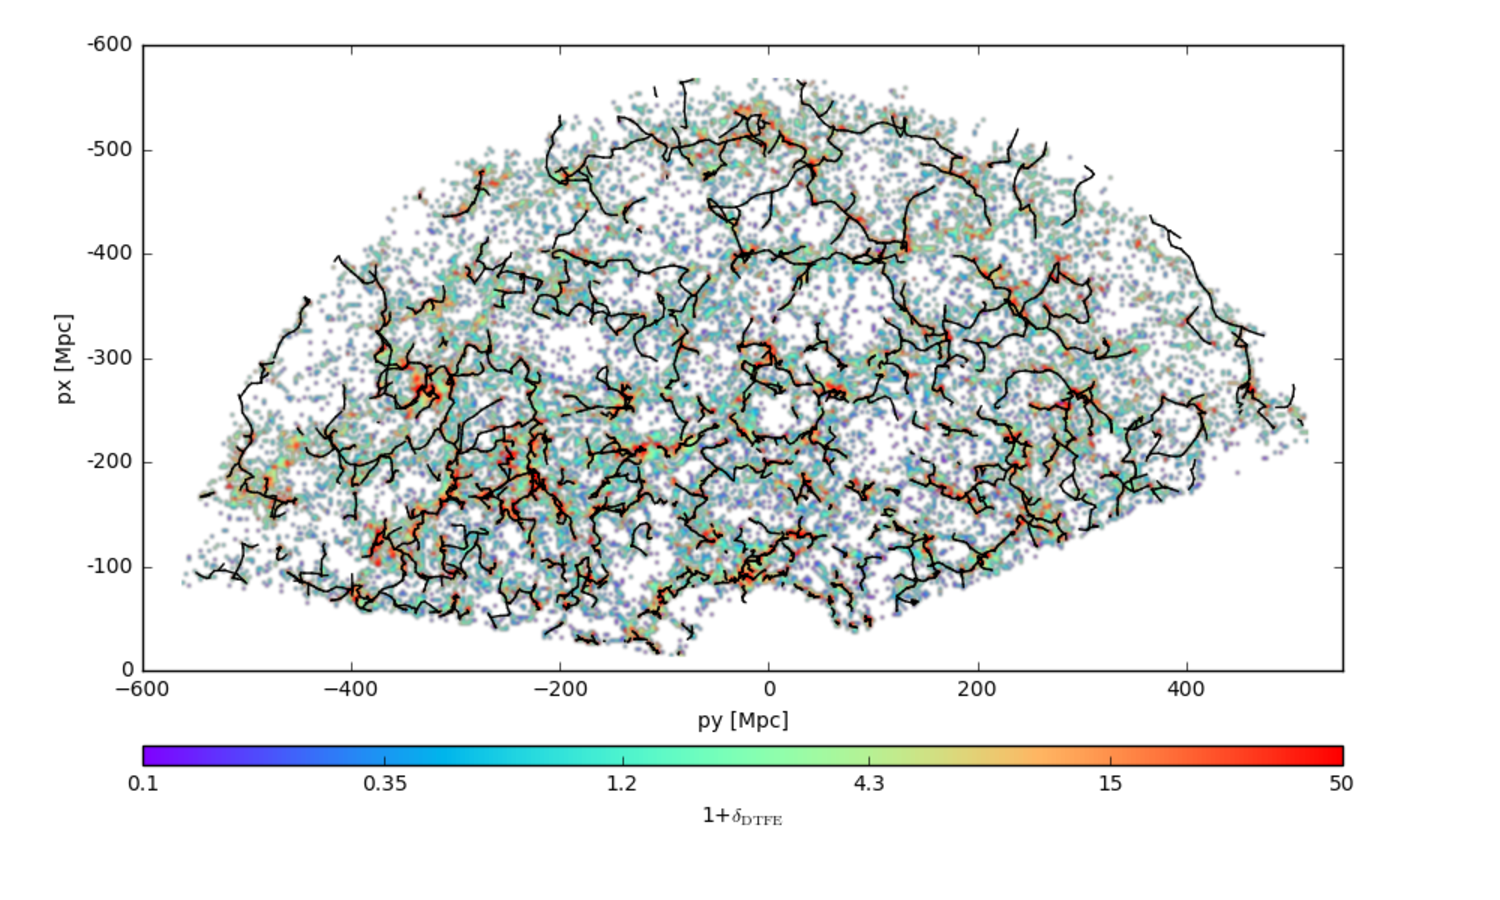
\includegraphics[width=\linewidth]{thesis/latex/halo_assembly_manga/SDSS_CW_DisPerSE.pdf}
    \caption[Illustration of the filamentary network for a slice of the SDSS field.]{Illustration of the filamentary network (black lines) for a slice of the SDSS field ($0.02 \leq z \leq 0.15$; $ 27 \leq$ dec $\leq 33$) extracted using the DisPerSE code. Only filamentary structures which are seen to persist above the 5$\sigma$ threshold are shown, along with the density contrast of the galaxy population. The density contrast is estimated using the small-scale DTFE estimator (see text). Adapted from \citet{duckworth2019_halo}, with credit to K. Kraljic.}
    \label{fig:disperse_sdss}
\end{figure*}

In observations we have an additional difficulty since we are not working with exact three dimensional positions in real space, however, in redshift space. To recover the intrinsic galaxy position, an estimation for the peculiar velocity must be made for each galaxy. On large-scales this corresponds to the Kaiser effect \citep{kaiser1987}, which acts to increase the contrast of the skeleton due the coherent motion of galaxies with the growth of structure \citep[e.g.][]{shi2016}. On small-scales, however, the Fingers of God effect \citep[FOG;][]{jackson1972,tulley1978} derives from random motions of galaxies within virialized haloes. The latter can elongate structure in redshift space leading to erroneous identification of filaments. We correct for the FOG effect using the technique outlined in \citet{kraljic2018}. In Figure \ref{fig:disperse_sdss} we show an example of the recovered density field from a set of galaxy positions in SDSS and the corresponding ridge extraction (i.e. filament detection). 

\section{Angular momentum in galaxies} \label{sec:ang_mom_intro}
\subsection{Turning out}
Angular momentum is one of the key properties that quantifies a galaxy. As galaxies form from the cooling and condensation of the initial gas cloud within dark matter haloes \citep{white1978, mo1998}. In the basic picture, the angular momentum content of the galaxy is inherited from the surrounding halo \citep[][]{fall1980}. In turn, this is acquired through tidal torques in the early growth phase from the large-scale structure \citep[e.g.][]{peebles1969, Doroshkevich1970}. If gravitational collapse proceeds unhindered, the initial gas cloud will form a stable rotating disc which eventually evolves into the late type galaxies (LTGs) we observe today \citep{white1978}. Since stars form from the rotating gas, the natural expectation is that they will inherit its dynamical characteristics often leading to coherent rotation between dark matter, gas and stars in both magnitude and direction. However, in the non-linear regime there is good reason to believe that the rotation of dark matter, gas and stars may decouple from each other as galaxies evolve up-to $z=0$. 

The evolution of a galaxy from initial collapse to today is seldom completed in isolation. By its very nature, small scale structure formation in $\Lambda$CDM is hierarchical with haloes undergoing bottom-up assembly from mergers of lower mass progenitors. In the non-linear regime, the angular momentum of the baryons in a galaxy can be driven dramatically away from the expectations of TTT through external processes such as interactions or mergers. How such interactions alter angular momentum depend on the magnitude, orientation and gas content of the merger. For example, gas rich mergers in general spin up galaxies whereas gas poor mergers are seen to spin down galaxies \citep[][]{lagos2017,lagos2018}.

\subsection{IFS surveys}
Developments in spectrographs have led to the advent of integral field spectroscopy (IFS) which provides spatially resolved spectra for galaxies. Unlike single-fibre galaxy surveys such as SDSS which only obtain spectra from the central $\sim 3 ''$ of a target galaxy, IFS observations enable spatially resolved spectral measurements up-to several effective radii (\re) across the faces of nearby galaxies. From these spectra, we can simultaneously extract kinematics of stars and gas, while obtaining absorption line strengths which provide radial gradients of gas phase metallicity and stellar population age. From this wealth of information, galaxy classification has evolved beyond visual morphologies, to consider dynamics of stars and gas, resolved star formation histories and stellar mass profiles. 

In kinematics, establishing work in the field has been the Spectrographic Areal Unit for Research on Optical Nebulae \citep[SAURON;][]{sauron} and ATLAS\textsuperscript{3D} \citep{atlas3d} surveys, which have focused on early type galaxies (ETGs) in the local Universe. IFS has enabled kinematic classification through a proxy for angular momentum based on the stellar kinematics up to one effective radius ($\mathrm{R_e}$). Termed $\mathrm{\lambda_{Re}}$, the measure enabled the clear distinction between slow and fast rotating ETGs \citep{emsellem2007, emsellem2011}. While there is still debate over whether 1$\mathrm{R_{e}}$ is large enough to fully encapsulate the complete kinematic morphology of a galaxy \citep{foster2013, arnold2014}, it has opened the door for understanding the relationship between optical morphology and angular momentum. 

IFS observations are costly, and such detailed information has often come at the cost of total galaxies observed. For example, in the last 10 years ATLAS\textsuperscript{3D} and CALIFA \citep{califa} observed 260 and 667 galaxies respectively with various selection criteria. IFS surveys for $\sim$1000 of galaxies across all optical morphologies are now a reality. For example, the Sydney-AAO  Multi-object  Integral  field  spectrograph  survey \citep[][]{croom2012, bryant2015} has mapped $\sim$3400 galaxies upto $z\sim0.12$ across a variety of environments. Even larger is the Mapping Nearby Galaxies at Apache Point \citep[MaNGA;][]{bundy2015, blanton2017} survey which will map $\sim$10000 galaxies in the local Universe ($z=0-0.15$). By design MaNGA will create a sample of near flat number density distribution across absolute $i$-band magnitude and stellar mass.

Recent studies in observations and simulations have demonstrated the close interlink between stellar angular momentum, stellar mass and morphology suggesting that late types and early type fast rotators form a continuous sequence rather than from fundamentally different formation pathways \citep[][]{cortese2016, lagos2017, graham2018}. First introduced by \citet{cappellari2011}, kinematic and morphological information can be combined to adapt Hubble's tuning fork into a \textit{comb} with an early-type handle and late-type bristles. An example of the comb can be found in Figure \ref{fig:ifu_comb} where the effective x-axis is based on rotational support. Remarkably, despite the highly non-linear processes involved, current cosmological surveys predict that the stellar angular momentum in rotationally supported galaxies at $z=0$ is still conserved from that of the dark matter halo \citep[e.g.][]{genel2015}. \red{subsection on morphology-density and rotational support?}

\begin{figure}
	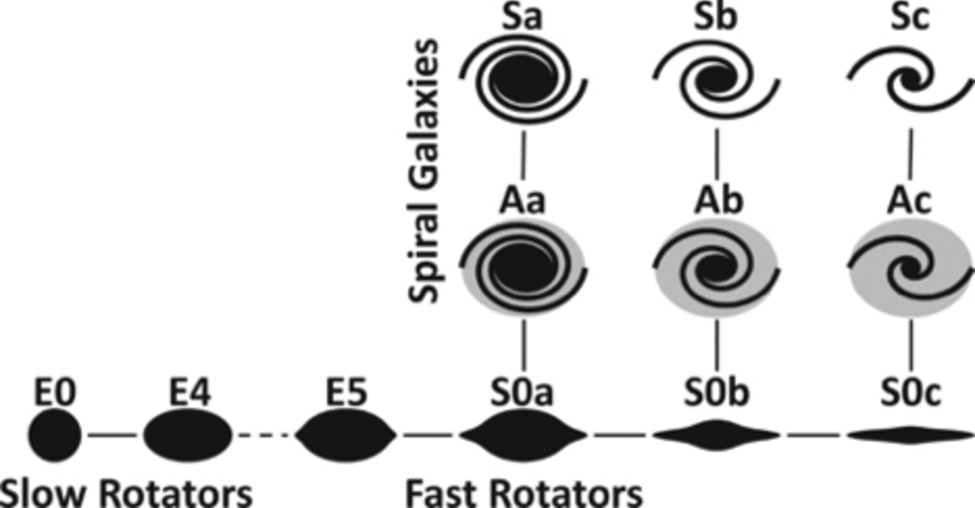
\includegraphics[width=\linewidth]{thesis/latex/introduction/ifu_comb.pdf}
    \caption{The kinematic comb classification from \citet{cappellari2011} where galaxies are divided based on a combination of their kinematic and morphological characteristics. The effective x-axis divides galaxies based on the degree of rotational support, going from slow (E0-4) to fast (E5-S0c) rotators. The effective y-axis divides galaxies on the degree of spiral structure, in parallel to the original tuning fork.}
    \label{fig:ifu_comb}
\end{figure}

\subsection{Angular momentum in the cosmic web}
As the baryonic gas flows within the gravitational potential well imposed by the web-like distribution of dark matter, material is advected giving rise to a fundamental connection between large scale structure and angular momentum in galaxies. Extending the formalism of TTT to include large scale structure formation \citep[e.g.][]{pichon2011, codis2015, laigle2015}, the angular momentum distribution of galaxies can be described relative to their neighbouring walls and filaments. In cosmological simulations, this can be seen as a mass dependent alignment between the spin of the dark matter haloes and the filament direction. The spin vectors of low mass haloes orient along the filament indicative of advection of angular momentum from the filament itself. Conversely high mass haloes have undergone mergers in the plane of the filament leading to a `flip' in orientation. How the spin of the haloes propogates to that of the baryonic components is complex and hence observations of this effect are inconclusive \citep[e.g.][]{tempel2013, krolewski2019, welker2020}. 

\section{Hydrodynamical simulations} \label{sec:hydro_sims_intro}
\subsection{Numerical methods}
In parallel with the advances in spectrographs leading to large scale IFS surveys, developments in both modelling and computing power have lead to numerical simulations driving forward understanding of galaxy formation and evolution. The establishment of the $\Lambda$CDM paradigm as the leading theory for our Universe, owes a lot to the development of pure dark matter N-body simulations. On cosmic scales, the formation of large scale structure can be well explained by the dynamics of dark matter (i.e. purely gravity), however, understanding the formation and evolution of galaxies is also reliant complex baryonic processes. Strong non-linear processes ranging from galaxy-galaxy mergers and interactions, feedback from both stars and black holes, to accretion of multiple gas phases, one certainty is that galaxies have difficult lives. Even more difficult is developing accurate physical models for each of these processes when simulating their impact.

In recent years, the first generation of cosmological \textit{hydrodynamical} simulations have helped understand the interplay between smaller scale baryonic processes and the anisotropy of the cosmic web, leading to the galactic diversity we observe. These `full-physics' simulations comprise of high-resolution dark matter N-body codes on cosmological volumes (100 Mpc and above) coupled with the hydrodynamics of gas and models for star formation and multiple feedback prescriptions. A non-exhaustive list of simulated Universes include \texttt{Horizon-AGN} \citep{dubois2014}, \texttt{EAGLE} \citep{schaye2015}, \texttt{Illustris} \citep{vogelsberger2014a, vogelsberger2014b, genel2014, sijacki2015}, \texttt{IllustrisTNG} \citep{marinacci18, naiman18, nelson18, pillepich18a, springel18}, and \texttt{SIMBA} \citep{dave2019}. \red{add more basics about simulations and general successes/failures.}

\subsection{Mocking the observers}
Ensuring that we are comparing apples to apples is a recurring theme when attempting to recover observations with simulations. De-convolving dissimilarity in how parameters are computed and physical differences in simulations is crucial in understanding how well observations are recovered. In the context of angular momentum and mass build up, recent work by \citet{sande2019} compare observations (SAMI, ATLAS\textsuperscript{3D}, CALIFA and MASSIVE surveys) to various predictions of hydrodynamical simulations (e.g. \texttt{EAGLE}; \citet{schaye2015}, \texttt{Horizon-AGN}; \citet{dubois2014}, \texttt{HYDRANGEA}; \citet{bahe2017}) at $z \sim 0$. Despite the vast improvement of cosmological simulations in recent years which broadly reproduce many galaxy relations, there are distinct differences in different stellar mass ranges for each simulation in each of physical size, shape and rotation with respect to observations.

Recent efforts to compare kinematics in simulations to observations include the \texttt{SimSpin} package \citep{harborne2019, harborne2020} who create a flexible framework to construct mock IFS observations from particle data in a range of simulations. With an emphasis on angular momentum, they provide a consistent methodology to compute observational properties such as $\lambda_R$ and $V/\sigma$ which is of particular relevance to the focus of this thesis.

\section{Halo assembly bias}
Bottom-up assembly in $\Lambda$CDM of dark matter haloes can be explained approximately by the excursion-set formalism which tracks the linear growth of primordial over-densities before spherically collapsing in the non-linear regime \citep{press1974,bond1991}. In the most basic form, environment is neglected and the assembly history of the halo is entirely dictated by its mass. This exclusive dependence on mass underlines the widely used halo occupation distribution \citep[HOD; e.g.][]{jing1998,peacock2000} modelling and various types of abundance matching \citep[e.g.][]{kravtsov2004,conroy2006}, which require galaxy clustering to be driven solely by halo mass \citep[e.g.][]{mo1996,sheth1999}. 

Parallel to the successes of HOD modelling, N-body simulations have fast converged on the fact that, at fixed halo mass, haloes which have formed at different times cluster differently \citep[e.g.][]{gao2005,wechsler2006,croton2007,wang2011}. Termed \textit{halo assembly bias}, this quantifies any physical quantity of a dark matter halo which correlates with halo clustering beyond the driving factor of halo mass. While most commonly considered as halo formation time, properties such as halo spin and concentration have also been demonstrated to be related with clustering \citep[e.g.][]{lacerna2012,lehmann2017}. 
Attempts to understand the origin of assembly bias have come from the large-scale tidal environment in which the given halo resides. Large-scale tidal forces are naturally anisotropic and intimately connected with the structure of the cosmic web. Halo assembly can therefore be de-convoluted as the influence of small and large scale forces. On small scales, gravity is dominant and the key properties are driven by local overdensity, encoded by the total mass of the halo. On large scales, the impact is more subtle \red{nuanced?}.

In simulations, \citet{hahn2009} found a systematic trend between halo formation time and the large-scale tidal force strength, derived from the geometric environment, at fixed halo mass. This effect is seen most strongly in low-mass haloes, arising from suppression of their growth when they reside within the vicinity of a much larger halo. This large halo acts to stop accretion on the low-mass halo in over-dense regions, effectively boosting the clustering of older low-mass haloes, compared to haloes of the same mass residing in under-dense regions that are less affected by tidal fields. \citet{ZOMGI} explore this phenomenon in the context of the cosmic web. Low-mass haloes residing within large filaments can often see their accretion `stalled' and hence will cease mass assembly earlier as matter flows preferentially along the filament to its densest points (nodes). Conversely low-mass haloes at the convergence point of multiple smaller filaments will have continued isotropic accretion resulting in longer continued mass growth and more recent formation. \citep[See][for a theoretical approach]{musso2018}.

Galaxies are our primary resource in probing the spatial distribution of dark matter. Their formation and subsequent evolution is tied to the assembly history of their host halo, however, determining the exact link is difficult. The observational counterpart of assembly bias is therefore tricky to isolate and as such is rightfully still under debate. In the context of galaxy evolution, the question of halo assembly bias can be rephrased to; \textit{does the cosmic web significantly impact galaxy evolution once stellar (or halo) mass has been accounted for?}

Early studies, however, have demonstrated observations of halo assembly bias. For example, \citet{tojeiro2017} compare a halo age proxy with respect to large-scale tidal environment defined in the Galaxy And Mass Assembly \citep[GAMA;][]{driver2009, driver2011} survey. They quantify tidal strength using the geometric classification of \citet{eardley2015} to characterise regions into geometric voids, sheets, filaments and knots corresponding to zero, one, two and three dimensions of collapse respectively. They find that low-mass haloes ($\lesssim 10^{12.5} M_{\odot}$) show a steadily increasing ratio of central galaxy stellar mass to total halo mass, corresponding to increasing halo age in regions of increasing tidal force strength (i.e. going from voids to knots). They find a tentative reversal of this trend for high-mass haloes ($\gtrsim 10^{13.2} M_{\odot}$). \citep[See][who explicitly look for changes in halo to stellar mass ratio with geometric environment using stacked lensing profiles, but find no significant changes when averaging over halo mass.]{brouwer2016}.

The tidal field can also be described in a topological sense with respect to the cosmic web. \citet{kraljic2018} provide an investigation in the GAMA survey through identification of the cosmic web, using the DisPerSE code. They estimate distances to nodes, filaments and walls as a function of galaxy properties such as $u - r$ colour, specific star formation rate (sSFR) and stellar mass. They find distinct gradients with more massive, redder (passive) galaxies residing closer to nodes, filaments and walls, indicative of mass dependent clustering. Additionally, at fixed stellar mass, both star formation rate (SFR) decreases and colour reddens for galaxies closer to both nodes and filaments. Assuming the flow of baryonic accretion follows that of dark matter, this observation is consistent with the `stalling' of haloes due to tidal environment.

\section{This thesis}
In this thesis, I want to help answer three questions:

\begin{itemize}
    
    \item Why does the rotation of ionized gas decouple from the overall rotation of a galaxy, and how is this related to the angular momentum content of the dark matter halo?
    
    \item Are signatures of halo assembly bias detectable in galaxy observables such as kinematic misalignment or galaxy spin? \red{maybe rephrase this question?}
    
    \item How does the anisotropy of the cosmic web impact both the kinematics within galaxies and the dynamics of galaxies in the larger potential well of the overall halo?
    
\end{itemize}

In Chapter 2, I introduce the concept of kinematic misalignment and its background in large scale Integral Field Spectroscopic surveys, before using observational sample of misaligned galaxies to understand their typical characteristics and fundamental relationships with other observable properties. In Chapter 3, I introduce a mock observational sample created from a cosmological scale hydrodynamical simulation to understand if the observational trends can be reproduced and what can be learned from their evolutionary histories. In Chapter 5, I investigate the relationship between black hole activity in this mock sample and the relationship with kinematic misalignment. In Chapter 6, I investigate if kinematic misalignment in observations can be related to various measures of the assembly history of the surrounding dark matter halo. In Chapter 7, I investigate the differences between the orbits of satellite galaxies in different environments of the cosmic web and the potential for this to be recovered by dynamical models. In Chapter 8, I present results relating the spin alignment of galaxies with large scale structure in a large scale Integral Field Spectroscopic survey. In Chapter 9, I relate the angular momentum content of galaxies and dark matter haloes to the initial conditions of a hydrodynamical simulation.